\chapter{Linear Dimensionality Reduction}

As presented in the previous sections, data sets with many features may present a series of issues: difficult visualization, high performance requirements, noise etc. In this section, it will be discussed methods related with linear dimensionality reduction, i.e., the shrinking of data sets by transformation and/or removal of features, while minimizing information loss.

Consider the synthetic data set $\vect K$. $\vect K$ has its samples expressed by two similarly scaled dimensions. It is clear, however, that the samples follow a very particular distribution:

\begin{figure}[H]
    \centering
	\captionsetup{justification=centering}

	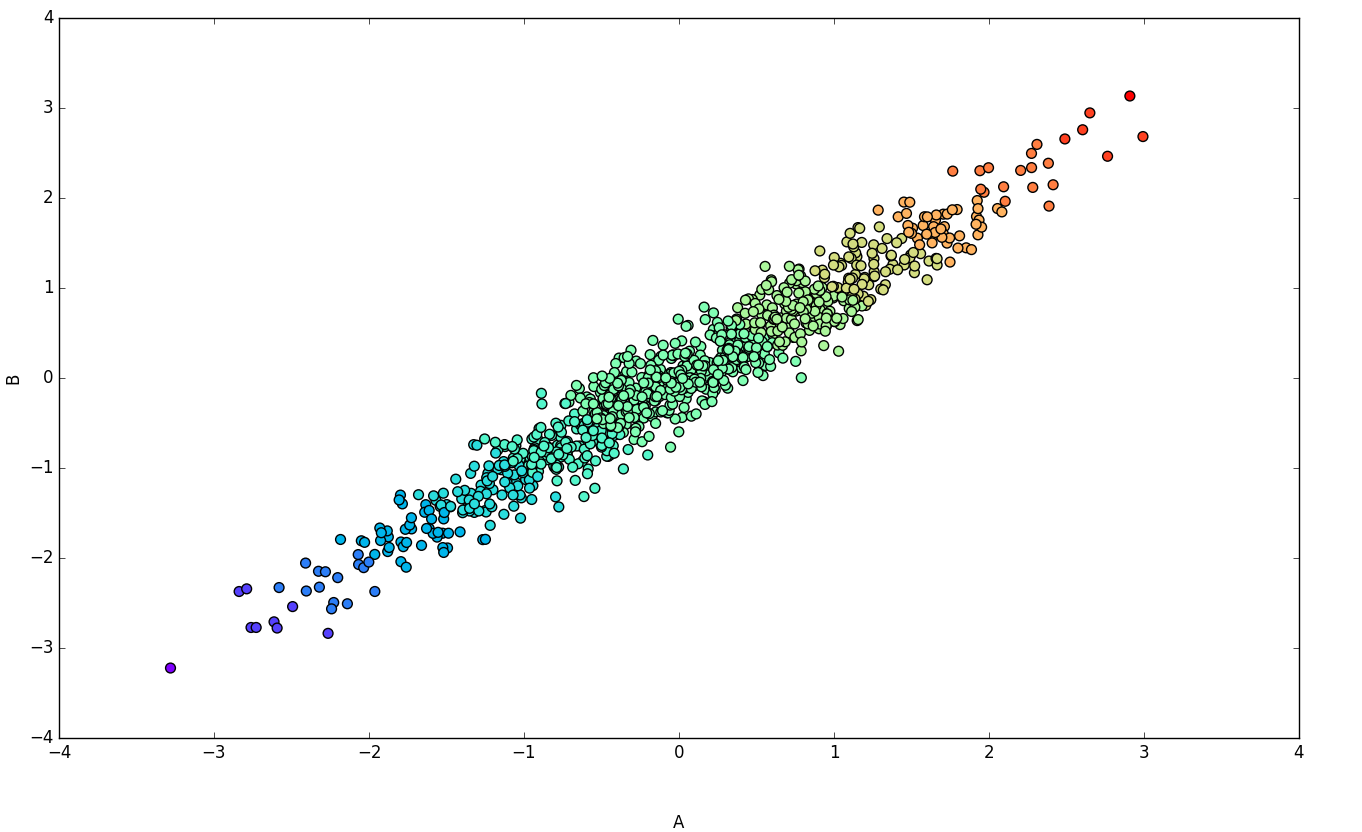
\includegraphics[width=.8\linewidth]{datasets/r}
	\caption{The data set $\vect K \in \mathbb{R}^n \times \mathbb{R}^n$.}
	\label{fig:datasetr}
\end{figure}

Additionally, something interesting can be observed when analyzing the covariance matrix of $K$: as it is not a diagonal matrix, the variance of $x$ from its mean somehow correlates with the variance of $y$ \cite{pcajon2003}.

\begin{table}[H]
	\centering
	\begin{tabular}{|c|c|c|}
		\hline
			& \textbf{x} & \textbf{y} \\\hline
		\textbf{x} & 1.26682132  & 1.29158697 \\\hline
		\textbf{y} & 1.29158697  & 1.40358478 \\\hline
	\end{tabular}
	\caption{Covariance between the components of $\vect K$.}
\end{table}

\section{Principal Component Analysis}

As in $K$, some data sets follow certain distributions that are majorly contained in a few orthogonal components, where a component is the result of a linear combination of the original features.

Principal Component Analysis (PCA) is a statistical technique that attempts to transform a $n$-dimensional data set $\vect X$ into a $m$-dimensional data set $\vect Y$, where, hopefully, $m \ll n$. Furthermore, the dimensions of $\vect Y$ will necessarily be orthogonal components aligned with the direction in which the variance of samples in $\vect X$ is maximum, commonly referred to as \textbf{principal components} \cite{pca1989}. In figure \ref{fig:datasetrpc}, the orange and purple arrows are the principal components of the data set $\vect K$.

\begin{figure}[H]
	\centering
	\captionsetup{justification=centering}
	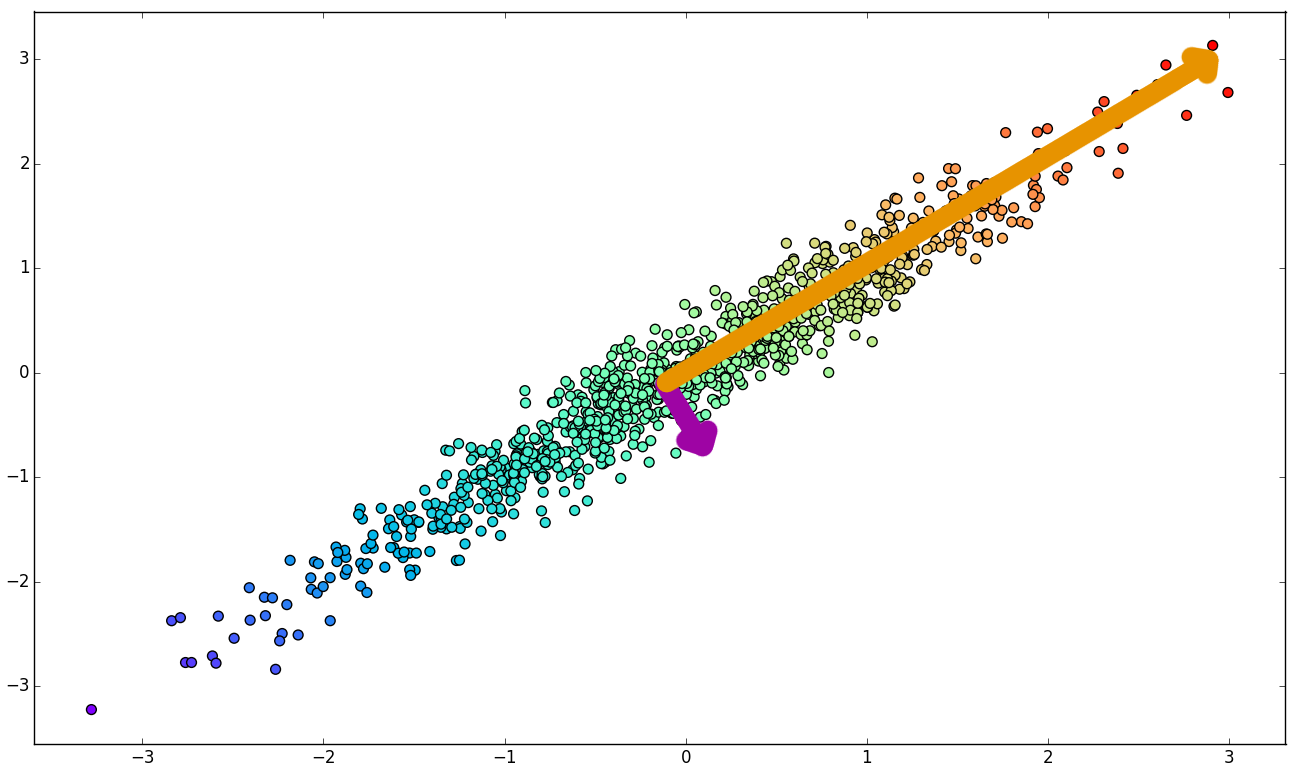
\includegraphics[width=.7\linewidth]{datasets/r_pcs}
	\caption{The principal components of $\vect K$ (orange and purple arrows).}
	\label{fig:datasetrpc}
\end{figure}

For a detailed experiment of reduction, learning and evaluation over the data set $\vect K$, see section \ref{experiments:k}.

\subsection{Study of the PCA Algorithm}

Let $\vect D$ be a dataset with $n$ samples and $f$ features and $\vect{X=HD}$, where $\vect H$ is the centering matrix. Our goal is to find which are the principal components of the covariance matrix $\vect \Sigma_X$:
\begin{align}
	\label{eq:pca-cov}
	\vect\Sigma_X=\frac{1}{n} \vect{X^\top X}
\end{align}

Using the \textbf{Singular Value Decomposition} method described in section \ref{sec:svd}, we known that
\begin{align}
	\label{eq:pca-svd}
	\vect{X = U\Sigma V^\top}
\end{align}

Needless to say, $\vect\Sigma$ is the diagonal matrix of singular values, not to be mistaken by the covariance matrix $\vect\Sigma_X$.

From \ref{eq:pca-cov} and \ref{eq:pca-svd}:
\begin{align*}
	\vect\Sigma_X &= \frac{1}{n} \vect{X^\top X} \\
	&= \frac{1}{n} \vect{(U\Sigma V^\top)^\top U\Sigma V^\top} \\
	&= \frac{1}{n} \vect{V\Sigma^2 V^\top}
\end{align*}

Which entails that $\vect V$ is the orthonormal matrix with $\vect\Sigma_X$'s eigenvectors as columns, where $\vect\Sigma$ contains the correspondent eigenvalues $\sigma_i^2$ associated with $v_i\in \vect V$ in its diagonal. Now notice that the principal components also spawn $\vect K$ it $\vect K$ is centered on the origin. Under these conditions, $\sigma_i v_i$ surely matches the $i$-th principal component. As we are interested in the dimensions that give most variance, we keep only the $m\in\mathbb{R}$ most significant eigenvalues and their correspondent eigenvectors.

Finally, it also worth remarking once again that the principal components are linear combinations of the original features (the canonical base) and $\vect V$ is the change-of-basis matrix from the generated base to the canonical. Naturally, $\vect V^{-1}$ is a change-of-basis matrix from the original space to the one that is generated by the principal components. Formally, if $x$ is a sample (row vector) from the $\vect X$ data set, its project $y$ is defined as:
\begin{align*}
	\vect{V y^\top} &= \vect x^\top \\
	\vect y^\top  &= \vect{V^{-1}x^\top}
\end{align*}

In the other hand, $\vect V$ is orthogonal, hence $\vect V^{-1}$ exists and it is equal to $\vect V^\top$:
\begin{align*}
	\vect y^\top &= \vect{V^\top x^\top} \\
	\vect y &= \vect{(V^\top x^\top)^\top} \\
      &= \vect{xV}
\end{align*}

\subsection{Formalization of the PCA Algorithm}

Let $\vect D$ be a data set with $n$ samples and $f$ features and $m\in\mathbb{R}$ the number of dimensions desired for the reduced data set \cite{pca2002, pcapy}.

\begin{enumerate}
	\item Find $\vect{X=HD}$, where $\vect H$ is the centering matrix.

	\item Calculate the covariance matrix $\vect\Sigma_X$.

	\item Use singular value decomposition to find the eigenvalues $\vect\Sigma = \{\sigma_i\}$ and eigenvectors $\vect V = \{v_i\}$ of $\vect\Sigma_X$.

	\item Sort the eigenvalues by their absolute value in descending order and select the first $m$ ones and their respective eigenvectors.
\end{enumerate}

\section{Multidimensional Scaling}

Alternatively to PCA, Multidimensional Scaling (or simply MDS) can be used to reduce the dimensionality of a data set. The method has, however, an extensive application domain and often appears in the literature in different contexts. An example of this is the problem of, given a set of objects $O$ and a dissimilarity measurement $\delta_{rs}, \forall (r, s) \in O\times O$, finding a suitable representation in the $\mathbb{R}^n$ for the objects in $O$ \cite{cox2001}.

For this project, we study the \textbf{classic MDS}. That is, when the dissimilarities considered are the Euclidean distances between coordinates in the $\mathbb{R}^n$, equivalating the method to PCA.

\subsection{Study of the MDS}

Let $\vect \Delta = [\delta_{rs}]_{n\times n}$ be the dissimilarity matrix, where $\delta_{rs}$ represents the Euclidean distances between two samples $\vect x_r, \vect x_s\in \mathbb{R}^m$ from the data set $[\vect X]_{n\times m}$ induced by the $L2$-norm. In other words,
\begin{align}
\label{eq:basemds}
\begin{split}
  \delta_{rs}  &= \sqrt{\sum_i (x_{ri}-x_{si})^2} \\
  &\iff \\
  \delta_{rs}^2 &= \sum_i (x_{ri}-x_{si})^2 \\
  &= (\vect{x_r-x_s}) \cdot (\vect{x_r-x_s}) \\
  &= \vect{x_r\cdot x_r + x_s\cdot x_s -2x_r\cdot x_s}
\end{split}
\end{align}

Now consider the matrix $\vect{B=XX^\top}$, where $b_{rs}=\vect x_{.r}\cdot \vect x_{.s}$. $\vect B$ can be decomposed as $\vect{U\Sigma U^\top} = \vect U \vect\Sigma^\frac{1}{2} \vect\Sigma^\frac{1}{2} \vect U^\top=\vect U \vect\Sigma^\frac{1}{2} (\vect U \vect\Sigma^\frac{1}{2})^\top = \vect{XX^\top}\iff \vect{X=U} \vect\Sigma^\frac{1}{2}$. If $\vect B$ can be derived from \ref{eq:basemds}, the problem is reduced to simply decompose $\vect B$ and using its eigenvalues and eigenvectors (similarly to what was done in PCA) to construct the data set $\vect Y$ \cite{cox2001}.

Firstly, we will assume that $\vect Y$ is centered in the origin (i.e., $\vect Y$ has its features' means equal to zero):
\begin{align}
	\label{eq:mds_zeromean}
	\sigma_f = \sum_i y_{if} = 0, \forall f\in [0, m)
\end{align}

Now, \ref{eq:basemds} $\implies$
\begin{align}
\label{eq:xsderivation}
\begin{split}
\frac{1}{n} \sum_r \delta_{rs}^2
&= \frac{1}{n} \sum_r (\vect x_r \cdot \vect x_r + \vect x_s\cdot \vect x_s -2 \vect x_r\cdot \vect x_s) \\
&= \frac{1}{n} \sum_r \vect x_r\cdot \vect x_r + \sum_r \vect x_s\cdot \vect x_s -2 \sum_r \vect x_r \cdot \vect x_s \\
&= \frac{1}{n} \sum_r \vect x_r\cdot \vect x_r + \sum_r \vect x_s\cdot \vect x_s -2 (\sum_r \vect x_r) \cdot \vect x_s \\
&= \frac{1}{n} \sum_r \vect x_r\cdot \vect x_r + n \vect x_s\cdot \vect x_s -2 (\vect 0) \cdot \vect x_s \\
&= \frac{1}{n} \sum_r \vect x_r\cdot \vect x_r + \vect x_s\cdot \vect x_s \\
&\iff \\
\vect x_s\cdot \vect x_s &= \frac{1}{n} (\sum_r \delta_{rs}^2 - \sum_r \vect x_r \cdot \vect x_r)
\end{split}
\end{align}

Similarly, to \ref{eq:xsderivation}:
\begin{align}
\label{eq:xrderivation}
\begin{split}
\vect x_r\cdot \vect x_r &= \frac{1}{n} (\sum_s \delta_{rs}^2 - \sum_s \vect x_s \cdot \vect x_s)
\end{split}
\end{align}

Putting \ref{eq:xsderivation} and \ref{eq:xrderivation} back in \ref{eq:basemds}:
\begin{align}
\label{eq:xrsderivation}
\begin{split}
\delta_{rs}^2 &= \frac{1}{n} (\sum_s \delta_{rs}^2 - \sum_s \vect x_s \cdot \vect x_s + \sum_r \delta_{rs}^2 - \sum_r \vect x_r \cdot \vect x_r) -2 \vect x_r \cdot \vect x_s \\
&\implies \\
\vect x_r\cdot \vect x_s &= -\frac{1}{2} (\delta_{rs}^2 - \frac{1}{n} [\sum_s \delta_{rs}^2 - \sum_s \vect x_s \cdot \vect x_s + \sum_r \delta_{rs}^2 - \sum_r \vect x_r \cdot \vect x_r])\\
&= -\frac{1}{2} (\delta_{rs}^2 - \frac{1}{n} [\sum_s \delta_{rs}^2 + \sum_r \delta_{rs}^2 - 2\sum_r \vect x_r \cdot \vect x_r])\\
\end{split}
\end{align}

To eliminate the $\vect{x_r\cdot x_r}$ term from \ref{eq:xrsderivation}:
\begin{align}
\label{eq:msd-xrr}
\begin{split}
\frac{1}{n^2} \sum_s\sum_r\delta_{rs}^2 &= \frac{1}{n^2} \sum_s\sum_r(\vect x_r \cdot \vect x_r + \vect x_s \cdot \vect x_s -2 \vect x_r \cdot \vect x_s) \\
&= \frac{1}{n^2}\sum_s(\sum_r \vect x_r \cdot \vect x_r + \sum_r \vect x_s \cdot \vect x_s -2\sum_r \vect x_r \cdot \vect x_s) \\
&= \frac{1}{n^2}\sum_s [\sum_r \vect x_r \cdot \vect x_r + \sum_r \vect x_s \cdot \vect x_s -2( \vect 0 \cdot \vect x_s)]\\
&= \frac{1}{n^2}\sum_s(\sum_r \vect x_r \cdot \vect x_r + n \vect x_s\cdot \vect x_s) \\
&= \frac{1}{n^2}(n \sum_r \vect x_r \cdot \vect x_r + n \sum_s \vect x_s \cdot \vect x_s) \\
&= \frac{1}{n^2} 2n \sum_r \vect x_r\cdot \vect x_r \\
&= \frac{2}{n} \sum_r \vect x_r \cdot \vect x_r
\end{split}
\end{align}

Finally, applying \ref{eq:msd-xrr} on \ref{eq:xsderivation}:
\begin{align}
\label{eq:mds-defb}
\begin{split}
\vect B_{rs} = \vect x_r\cdot \vect x_s = -\frac{1}{2} (\delta_{rs}^2 - \frac{1}{n} [\sum_s \delta_{rs}^2 + \sum_r \delta_{rs}^2 - \frac{1}{n}\sum_s \sum_r \delta_{rs}^2])
\end{split}
\end{align}

From \ref{eq:mds-defb}, it becomes clear that $\vect B$ is, in fact, the double centering of the matrix $\vect A=-\frac{1}{2}\vect \Delta^2$. I.e., $\vect B=\vect{HAH}$. Spectral decomposition can now be performed onto $\vect B$, resulting in the matrices $\vect \Sigma$ and $\vect U$.

Finally, in order to reduce the dimensionality of the embedding, we can sort the eigenvalues (and their respective eigenvectors, the columns of $\vect U$) in decrease order and keep only the ones that offer greater variance.

\begin{remark}
	As euclidean distances were used to build the dissimilarity matrix $\vect \Delta$, $\vect B$ is indubitably positive semidefinite, hence $\sigma_i \ge 0, \forall i\in [0, n)$. However, negative eigenvalues might appear if other dissimilarity measurement were to be used. In these cases, one might consider to simply ignore such components.
\end{remark}

\subsection{Formalization of the Multidimensional Scaling Method}

Let $\vect X$ be a data set with $n$ samples and $f$ features and $m\in\mathbb{R}$ the number of dimensions desired for the reduced data set \cite{cox2001}.

\begin{enumerate}
	\item Calculate the dissimilarity matrix $[\delta]_{rs}$, where $\delta_{rs} = \sqrt{\sum_i (x_{ri} - x_{si})^2}$
	\item Calculate the matrix $\vect A=-\frac{1}{2}\delta_{rs}^2$ and $\vect{B=HAH}$, where $\vect H$ is the centering matrix.

	\item Use spectral decomposition to find the matrices $\vect \Sigma$ and $\vect U$.

	\item Select the $m$ greatest eigenvalues in $\vect \Sigma$. From these, create the matrices $\vect \Sigma'=[\sigma'_{m\times m}]$ and $\vect U'=[u'_{n\times m}]$, where each column $i$ contains the eigenvector associated with $\sigma'_i$.

	\item Construct the $m$-dimensional embedding $\vect Y=\vect U'\vect \Sigma'^{\frac{1}{2}}$
\end{enumerate}

\section{Evaluating Reductions}

Although the factors that determine if a reduction is acceptable or not are often influenced by particularities of the problem in hand, the researcher's past experience with MDS and his judgment \cite{naes1996multivariate}, some measures were developed to attempt to somehow formalize it. One in particular, which recurrently appears in literature, is known as the \textbf{Kruskal's stress}.

Intuitively, Kruskal's stress \cite{naes1996multivariate} considers reductions that preserve dissimilarities between samples better that the ones which highly distort them. Formally, let $\vect X_{n \times f}$ be a data set with $n$ samples and $f$ dimensions, $\vect Y_{n \times p}$ its reduction to $p$ dimensions, and the dissimilarity measurements $\delta_{ij}$ and $\hat{\delta}_{ij}$ defined for all samples $i$ and $j$ in $\vect X$ and $\vect Y$, respectively:
\begin{align*}
	Stress &= [\frac{\sum_i \sum_j (\delta_{ij} - \hat{\delta}_{ij})^2}{\sum_i \sum_j \delta_{ij}^2}]^{\frac{1}{2}}
\end{align*}

From the formula above, {\em Stress} is visibly contained in the interval $[0, 1]$, where 0 represents the best possible fit (all dissimilarities are the same), while 1 represents the worse.
